\section{Результаты исследования}
\subsection{Dataset}
Для исследования былы подобранны изображения различных типов, для определения, к какми классам изображения
какие фильтры применять изображения. Имеются: фотографии архитектуры, текстуры, изображения с низкой освещенностью, портреты людей, а так же комбинация некоторых. Все изображения взяты с сайта https://pixabay.com/images/search/people/. Ниже приведены экземпляры изображений.
Изображение архитектуры:
\begin{figure}[h]
	%\center{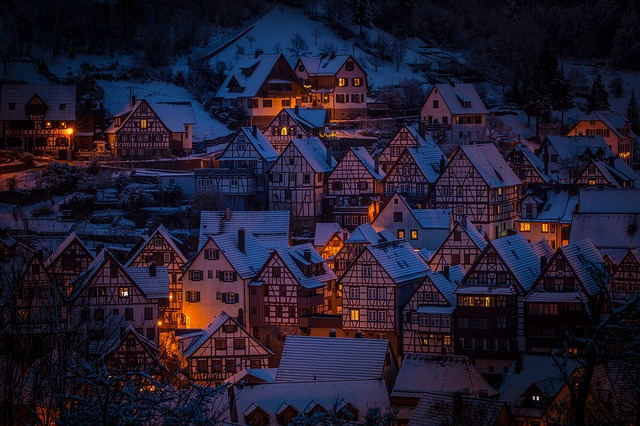
\includegraphics[width=0.4\textheight, keepaspectratio]{architecture-3076685_640.jpg}}
	\caption{изображение типа архитектура}
	\label{fig:Architecture}
\end{figure}
\begin{figure}[h]
	%	\center{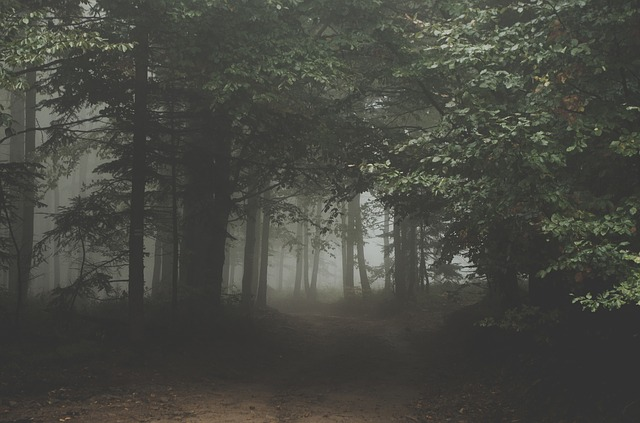
\includegraphics[width=0.4\textheight, keepaspectratio]{forest-1031022_640.jpg}}
	\caption{изображение типа плохое освещение}
	\label{fig:Night}
\end{figure}
\begin{figure}[h]
	%	\center{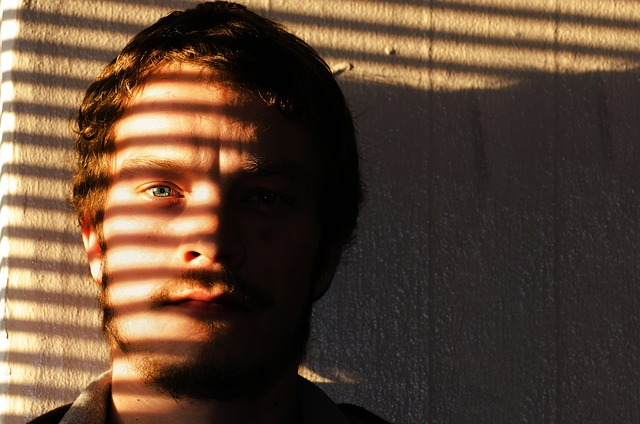
\includegraphics[width=0.4\textheight, keepaspectratio]{man-164962_640.jpg}}
	\caption{изображение типа портерт}
	\label{fig:Man}
\end{figure}
\begin{figure}[h]
	%	\center{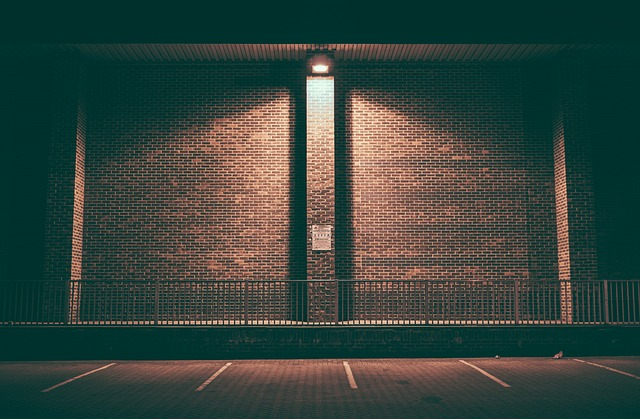
\includegraphics[width=0.4\textheight, keepaspectratio]{brick-wall-1834446_640.jpg}}
	\caption{изображение типа текстура}
	\label{fig:Texture}
\end{figure}
\begin{figure}[h]
	%	\center{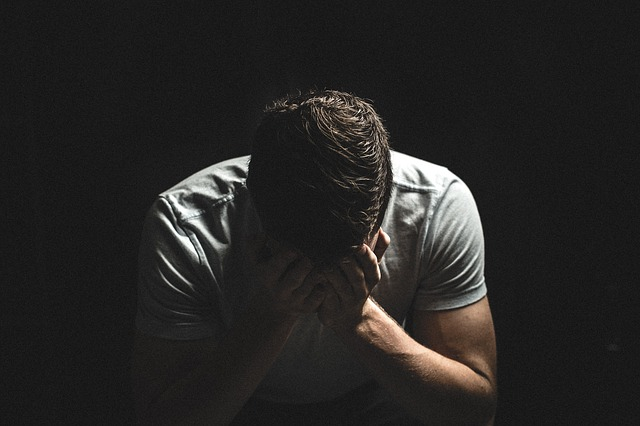
\includegraphics[width=0.4\textheight, keepaspectratio]{guy-2617866_640.jpg}}
	\caption{изображение типа текстура}
	\label{fig:Guy}
\end{figure}